% ---------------------------------------------------------------------------- %
\chapter{Vereinfachtes Modell f\"ur ein PV-Modul}
\label{app:models:develop:module:simple}
% ---------------------------------------------------------------------------- %

Zur  Reduktion des  Rechenaufwands im  Vergleich zu  dem im  vorigen Abschnitt
entwickelten Modell soll ein vereinfachtes Modell eines Solarmoduls entwickelt
werden.

Ausgangspunkt   ist   das   Eindiodenmodell    einer   Zelle   aus   Abbildung
\todo{reference}, f\"ur  welches die Parameter  so angepasst werden,  dass das
Verhalten des aus Zellen aufgebauten Modells aus dem vorigen Abschnitt und des
vereinfachten Modells zufriedenstellend \"ubereinstimmen.

Das Vorgehen ist dabei wie folgt: \todo{Eigentliche Werte}

\begin{itemize}
    \firmlist
    \item
        Die parasit\"are  Kapazit\"at des  Moduls wird angepasst  gem\"ass dem
        Gesetz zur Serieschaltung von Kapazit\"aten:
        $C_{\mathrm{p, Modul}} = C_{\mathrm{p, Zelle}} \div \text{Anzahl Zellen}$
    \item
        Der Seriewiderstand des Moduls ist die Summe der Seriewiderst\"ande aller
        Zellen
    \item
        Der  Parallele   Widerstand  wird   entsprechend  der   Anzahl  Zellen
        hochgerechnet.
        \todo{kein Einfluss, verifikation}
    \item
        Der Reverse  Saturation Current  des Moduls ist  von der  Fl\"ache des
        Moduls abh\"angig und  wird als Startwert vorerst  gem\"ass der Anzahl
        Module hochgerechnet.
    \item
        Der  Idealit\"atsfaktor   wird  vorerst  unver\"andert   belassen  und
        anschliessend iterativ angepasst.
\end{itemize}

Gem\"ass dieser Methodik werden die Startwerte festgelegt auf:

\begin{itemize}
    \firmlist
    \item
        $C_{\mathrm{p, Modul}} = \SI{167}{\nano\farad}$
    \item
        $R_{\mathrm{S}} = \SI{12}{\milli\ohm}$
    \item
        $R_{\mathrm{Shunt}} = \SI{60}{\kilo\ohm}$
    \item
        $I_{\mathrm{S}} = \SI{288}{\milli\ampere}$
    \item
        $n = 118$
\end{itemize}

Mit diesen  Werten werden verschiedene  Szenarien simuliert und  die Resultate
mit den  Ergebnissen des komplexeren Modells  verglichen. Durch Iteration wird
$I_{\mathrm{S}}$ schlussendlich  auf \SI{2.88}{\micro\ampere}  festgelegt.

Abbildungen
\ref{fig:model:simpel:verif:current:mosfet:freq},
\ref{fig:model:simpel:verif:voltage:mosfet:freq},
\ref{fig:model:simpel:verif:current:RL:freq} und
\ref{fig:model:simpel:verif:current:mosfet:time} stellen die Resultate
verschiedener Simulationen mit und ohne Last f\"ur das vereinfachte Modell und
das zellenbasierte  Modell graphisch dar.   Wie zu erkennen ist,  besteht eine
gute \"Ubereinstimmung. Es sind jeweils  die Kurve des komplexen Modul-Modells
(\textbf{\textcolor{magenta}{magenta}}) sowie die Kurve f\"ur das vereinfachte
Modell dargestellt (\textbf{\textcolor{blue}{blau}}).

Die   f\"ur    die   Simulationen    benutzten   Beschaltungen    der   Zellen
sind    in    den   Abbildungen    \ref{fig:model:simple:verif:circuit:noLoad}
und         \ref{fig:model:simple:verif:circuit:Load}        auf         Seite
\pageref{fig:model:simple:verif:circuit:Load} dargestellt.

%Parasit\"are Kapazit\"at: Kapazit\"at einer Zelle / anzahl Zellen \\
%Serie widerstand: widerstand einzelzelle * anzahl zellen \\
%shunt widerstand: widerstand einer zelle / anzahl zellen \\
%IS: IS einzelzelle * anzahl zellen (0.288m) -> anpassen, bis frequenzgang und zeitplot passend \\
%N: N einzelzelle * anzahl zellen \\
%Shockley diode model \\
\todo{Einheiten achsen, auflistung parameter}


\begin{figure}
    \begin{tikzpicture}
       \begin{scope}[x={(0mm,0mm)},y={(90mm,0.9\textwidth)}]
           \begin{axis}[%
                   xmode=log,
                   height=45mm,
                   width=0.9\textwidth,
                   at={(0,45mm)},
                   grid=both,
                   xlabel=Frequenz (\si{\hertz}),
                   ylabel=Strom (\si{\deci\bel}),
               ]
                \addplot[color=blue] table {data/simple-model-verification/module-72cells-series--reference--freq-sweep-over-mosfet-no-load--I--magn.dat};
                \addplot[color=magenta] table {data/simple-model-verification/module-simple-72x1--freq-sqeep-over-mosfet-no-load--I--magn.dat};
           \end{axis}
           \begin{axis}[%
                   xmode=log,
                   height=45mm,
                   width=0.9\textwidth,
                   at={(0,0)},
                   grid=both,
                   xlabel=Frequenz (\si{\hertz}),
                   ylabel=Phase (\si{\degree}),
               ]
                \addplot[color=blue] table {data/simple-model-verification/module-72cells-series--reference--freq-sweep-over-mosfet-no-load--I--phase.dat};
                \addplot[color=magenta] table {data/simple-model-verification/module-simple-72x1--freq-sqeep-over-mosfet-no-load--I--phase.dat};
           \end{axis}
       \end{scope}
   \end{tikzpicture}
    \caption{%
        Frequenzgang       des       Stroms       durch       den       MOSFET
        bei      einer      Beschaltung      ohne      zus\"atzliche      Last
        gem\"ass     Abbildung    \ref{fig:model:simple:verif:circuit:noLoad}.
        \textbf{\textcolor{magenta}{magenta}}:         einfaches        Modell
        \textbf{\textcolor{blue}{blau}}: komplexes Modell%
    }
    \label{fig:model:simpel:verif:current:mosfet:freq}
\end{figure}

\begin{figure}
    \begin{tikzpicture}
       \begin{scope}[x={(0mm,0mm)},y={(90mm,0.9\textwidth)}]
           \begin{axis}[%
                   xmode=log,
                   height=45mm,
                   width=0.9\textwidth,
                   at={(0,45mm)},
                   grid=both,
                   xlabel=Frequenz (\si{\hertz}),
                   ylabel=Spannung (\si{\deci\bel}),
               ]
                \addplot[color=blue] table {data/simple-model-verification/module-72cells-series--reference--freq-sweep-over-mosfet-no-load--U--magn.dat};
                \addplot[color=magenta] table {data/simple-model-verification/module-simple-72x1--freq-sweep-over-mosfet-no-load--U--magn.dat};
           \end{axis}
           \begin{axis}[%
                   xmode=log,
                   height=45mm,
                   width=0.9\textwidth,
                   at={(0,0)},
                   grid=both,
                   xlabel=Frequenz (\si{\hertz}),
                   ylabel=Phase (\si{\degree}),
               ]
                \addplot[color=blue] table {data/simple-model-verification/module-72cells-series--reference--freq-sweep-over-mosfet-no-load--U--phase.dat};
                \addplot[color=magenta] table {data/simple-model-verification/module-simple-72x1--freq-sweep-over-mosfet-no-load--U--phase.dat};
           \end{axis}
       \end{scope}
   \end{tikzpicture}
    \caption{%
        Frequenzgang      der       Spannung      \"uber       dem      MOSFET
        bei      einer      Beschaltung      ohne      zus\"atzliche      Last
        gem\"ass     Abbildung    \ref{fig:model:simple:verif:circuit:noLoad}.
        \textbf{\textcolor{magenta}{magenta}}:         einfaches        Modell
        \textbf{\textcolor{blue}{blau}}: komplexes Modell%
    }
    \label{fig:model:simpel:verif:voltage:mosfet:freq}
\end{figure}

\begin{figure}
    \begin{tikzpicture}
       \begin{scope}[x={(0mm,0mm)},y={(90mm,0.9\textwidth)}]
           \begin{axis}[%
                   xmode=log,
                   height=45mm,
                   width=0.9\textwidth,
                   at={(0,45mm)},
                   grid=both,
                   xlabel=Frequenz (\si{\hertz}),
                   ylabel=Spannung (\si{\deci\bel}),
               ]
                \addplot[color=blue] table {data/simple-model-verification/module-72cells-series--reference--freq-sweep-over-Rload--100ohm-100uF--I--magn.dat};
                \addplot[color=magenta] table {data/simple-model-verification/module-simple-72x1--freq-sweep-over-Rload--100ohm-100uF--I--magn.dat};
           \end{axis}
           \begin{axis}[%
                   xmode=log,
                   height=45mm,
                   width=0.9\textwidth,
                   at={(0,0)},
                   grid=both,
                   xlabel=Frequenz (\si{\hertz}),
                   ylabel=Phase (\si{\degree}),
               ]
                \addplot[color=blue] table {data/simple-model-verification/module-72cells-series--reference--freq-sweep-over-Rload--100ohm-100uF--I--phase.dat};
                \addplot[color=magenta] table {data/simple-model-verification/module-simple-72x1--freq-sweep-over-Rload--100ohm-100uF--I--phase.dat};
           \end{axis}
       \end{scope}
   \end{tikzpicture}
   \caption{%
       Frequenzgang   des   Stroms   durch  den   Lastwiderstand   bei   einer
       Last    von   \SI{100}{\ohm}    parallel   zu    \SI{100}{\micro\farad}
       gem\"ass      Abbildung      \ref{fig:model:simple:verif:circuit:Load}.
       \textbf{\textcolor{magenta}{magenta}}:         einfaches         Modell
       \textbf{\textcolor{blue}{blau}}: komplexes Modell%
    }
    \label{fig:model:simpel:verif:current:RL:freq}
\end{figure}

\begin{figure}
    \begin{tikzpicture}
       \begin{scope}[x={(0mm,0mm)},y={(60mm,0.9\textwidth)}]
           \begin{axis}[%
                   height=60mm,
                   width=0.9\textwidth,
                   at={(0,0)},
                   grid=both,
                   xlabel=Zeit (\si{\second}),
                   ylabel=Strom (\si{\ampere}),
               ]
                \addplot[color=blue] table {data/simple-model-verification/module-72cells-series--reference--time-domain-over-mosfet-10kHz--I.dat};
                \addplot[color=magenta] table {data/simple-model-verification/module-simple-72x1--time-domain-over-mosfet--10kHz--I.dat};
           \end{axis}
       \end{scope}
   \end{tikzpicture}
    \caption{%
        Zeitlicher     Verlauf     des     Stroms     durch     den     MOSFET
       bei      einer      Beschaltung       ohne      zus\"atzliche      Last
       gem\"ass     Abbildung     \ref{fig:model:simple:verif:circuit:noLoad}.
       \textbf{\textcolor{magenta}{magenta}}:         einfaches         Modell
       \textbf{\textcolor{blue}{blau}}: komplexes Modell%
    }
    \label{fig:model:simpel:verif:current:mosfet:time}
\end{figure}

\begin{figure}[h!tb]
    {\centering
    \adjustbox{valign=b}{%
        \begin{minipage}{0.475\textwidth}
            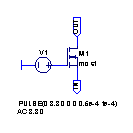
\includegraphics[width=\textwidth]{images/ltspice/module-test-circuit-without-load.eps}
            \caption{%
                Schaltung         zur         Simulation         ohne         Last
                (Abbildungen     \ref{fig:model:simpel:verif:current:mosfet:freq},
                \ref{fig:model:simpel:verif:voltage:mosfet:freq}               und
                \ref{fig:model:simpel:verif:current:mosfet:time}). Die  Zelle wird
                mit einem Transistor  kurzgeschlossen.  Die \textbf{\code{IN}} und
                \textbf{\code{OUT}}-Terminals  entsprechen  den Anschl\"ussen  des
                Solarmoduls  in  Abbildung \ref{fig:ltspice:module:simple}  (Seite
                \pageref{fig:ltspice:module:simple}) f\"ur das vereinfachte Modell
                und   Abbildung   \ref{fig:ltspice:module:cellBased:72x1}   (Seite
                \pageref{fig:ltspice:module:cellBased:72x1})  f\"ur  das  komplexe
                Modell mit 72 Zellen in Serie.%
            }
            \label{fig:model:simple:verif:circuit:noLoad}
        \end{minipage}%
    }\hspace*{0.05\textwidth}\adjustbox{valign=b}{%
        \begin{minipage}{0.475\textwidth}
            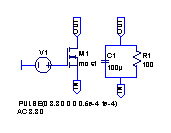
\includegraphics[width=\textwidth]{images/ltspice/module-test-circuit-with-load.eps}
            \caption{%
                Schaltung   zur   Simulation   mit   resistiver/kapazitiver   Last
                (Abbildung   \ref{fig:model:simpel:verif:current:RL:freq}).    Die
                Zelle     wird    mit     einem    Transistor     kurzgeschlossen.
                Die    \textbf{\code{IN}}     und    \textbf{\code{OUT}}-Terminals
                entsprechen      den       Anschl\"ussen      des      Solarmoduls
                in      Abbildung      \ref{fig:ltspice:module:simple}      (Seite
                \pageref{fig:ltspice:module:simple}) f\"ur das vereinfachte Modell
                und   Abbildung   \ref{fig:ltspice:module:cellBased:72x1}   (Seite
                \pageref{fig:ltspice:module:cellBased:72x1})  f\"ur  das  komplexe
                Modell mit 72 Zellen in Serie.%
            }
            \label{fig:model:simple:verif:circuit:Load}
        \end{minipage}%
    }}
    \vspace*{1em}
    Das benutzte \code{LTspice}-Modell f\"ur den MOSFET ist:\\
    \code{.model  mos1   VDMOS(Rg=3  Vto=1.7  Rd=8m  Rs=6m   Rb=10m  Kp=70
    Cgdmax=2.5n Cgdmin=.4n Cgs=2n Cjo=1n Is=80p Vds=100 Ron=20m Qg=40n)}%
\end{figure}

